\documentclass{beamer}
\usepackage{listings}
\lstset{
%language=C,
frame=single, 
breaklines=true,
columns=fullflexible
}
\usepackage{subcaption}
\usepackage{url}
\usepackage{tikz}
\usepackage{tkz-euclide} % loads  TikZ and tkz-base
%\usetkzobj{all}
\usetikzlibrary{calc,math}
\usepackage{float}
\newcommand\norm[1]{\left\lVert#1\right\rVert}
\providecommand{\pr}[1]{\ensuremath{\Pr\left(#1\right)}}
\providecommand{\sbrak}[1]{\ensuremath{{}\left[#1\right]}}
\providecommand{\brak}[1]{\ensuremath{\left(#1\right)}}
\providecommand{\fourier}{\overset{\mathcal{F}}{ \rightleftharpoons}}
\providecommand{\ztrans}{\overset{\mathcal{Z}}{ \rightleftharpoons}}
\providecommand{\abs}[1]{\left\vert#1\right\vert}
\renewcommand{\vec}[1]{\mathbf{#1}}
\usepackage[export]{adjustbox}
\usepackage[utf8]{inputenc}
\usepackage{amsmath}
\usetheme{Boadilla}

\title{GATE EC 2001 - Q.16}
\author{Tanmay Goyal - AI20BTECH11021}

\date{}

\begin{document}

\begin{frame}
\titlepage
\end{frame}
\begin{frame}
\frametitle{Question}
\begin{flushleft} 
\begin{columns}
\begin{column}{0.5\textwidth}
\begin{figure}[!ht]
\centering
 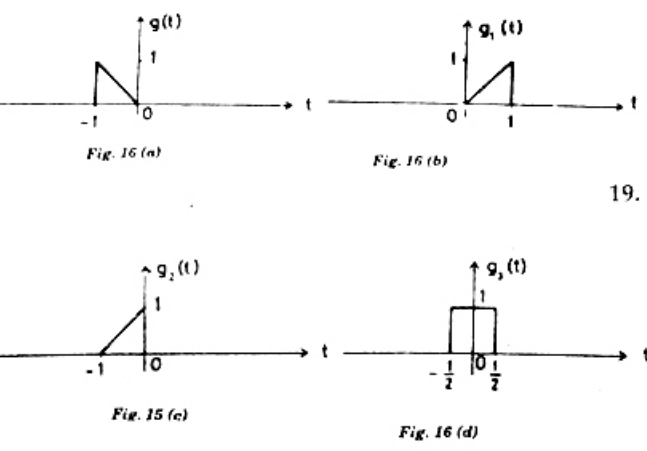
\includegraphics[width=\columnwidth]{Question.png}
\end{figure}
\end{column}
\begin{column}{0.5\textwidth}
The Fourier Transform $G(\omega)$ of the signal $g(t)$ is given by 
\begin{align}
    G(\omega) = \frac{1}{\omega^2}(e^{j\omega} - j\omega e^{j\omega} - 1)
\end{align}
Using this information, find the Fourier Transforms of the signals $g_1(t)$, $g_2(t)$ and $g_3(t)$.
\end{column}
\end{columns}
\end{flushleft}
\end{frame}

\begin{frame}[fragile]
\frametitle{Result of Time Shifting on Fourier Transform}

\begin{flushleft}
\begin{lemma}
If 
\begin{align}
    g(t) \fourier G(\omega)
\end{align}
then,
\begin{align}
    g(t \pm t_0) \fourier G(\omega)e^{\pm j\omega t_0}
\end{align}
\label{shift}
\end{lemma} 
\begin{proof}
We know, 
\begin{align}
    G(\omega) = \int_{-\infty}^\infty g(t) e^{-j \omega t} \,dt
\end{align}
\end{proof}
\end{flushleft}
\end{frame}


\begin{frame}[fragile]
\frametitle{Proof continued}
\begin{flushleft}

\begin{proof}
Let
\begin{align}
    g(t + t_0) \fourier G'(\omega)
\end{align}
Then, 
\begin{align}
    G'(\omega) = \int_{-\infty}^\infty g(t + t_0) e^{-j \omega t} \,dt
\end{align}
Substituting $t + t_0 = T$, we get:
\begin{align}
    G'(\omega) = \int_{-\infty}^\infty g(T) e^{-j \omega (T - t_0)} \,dT\\
      =e^{j \omega t_0} \int_{-\infty}^\infty g(T) e^{-j \omega T} \,dT\\
       = e^{j \omega t_0}G(\omega)
\end{align}
\end{proof}
\end{flushleft}
\end{frame}


\begin{frame}[fragile]
\frametitle{Result of Time scaling on Fourier Transform}
\begin{flushleft}
\begin{lemma}
If 
\begin{align}
    g(t) \fourier G(\omega)
\end{align}
then,
\begin{align}
    g(\alpha t) \fourier \frac{1}{\abs{\alpha}}G\brak{\frac{\omega}{\alpha}}
\end{align}
\label{scale}
\end{lemma}
\begin{proof}
Consider $\alpha > 0$. Then, we know, 
\begin{align}
    G(\omega) = \int_{-\infty}^\infty g(t) e^{-j \omega t} \,dt
\end{align}
\end{proof}
\end{flushleft}

\end{frame}


\begin{frame}[fragile]
\frametitle{Proof Continued}
\begin{flushleft}
\begin{proof}
Let 
\begin{align}
    g(\alpha t) \fourier G'(\omega)
\end{align}
Then,
\begin{align}
    G'(\omega) = \int_{-\infty}^\infty g(\alpha t) e^{-j \omega t} \,dt
\end{align}
Making the substitution $T = \alpha t$, we get:
\begin{align}
     G'(\omega) = \frac{1}{\alpha}\int_{-\infty}^\infty g(T) e^{-j \frac{\omega T}{\alpha}} \,dT\\
     = \frac{1}{\alpha}G\brak{\frac{\omega}{\alpha}}
\end{align}
\end{proof}
\end{flushleft}

\end{frame}

\begin{frame}[fragile]
\frametitle{Effect of Time Reversal on Fourier Transform}
\begin{flushleft}
\begin{corollary}
If 
\begin{align}
    g(t) \fourier G(\omega)
\end{align}
then,
\begin{align}
    g(- t) \fourier G(-\omega)
\end{align}
\label{reverse}
\end{corollary}
\end{flushleft}

\end{frame}

\begin{frame}[fragile]
\frametitle{Differentiation of Fourier Transform in Time Domain}
\begin{flushleft}
\begin{lemma}
If 
\begin{align}
    g(t) \fourier G(\omega)
\end{align}
then,
\begin{align}
    \frac{d g(t)}{dt} \fourier (j\omega) G(\omega)
\end{align}
\label{diff}
\end{lemma}
\end{flushleft}

\end{frame}


\begin{frame}[fragile]
\frametitle{Proof}
\begin{flushleft}

\begin{proof}
Using the formula for Inverse Fourier transform, we know:
\begin{align}
    g(t) = \frac{1}{2\pi}\int_{-\infty}^{\infty}G(\omega)e^{j\omega t} \,d\omega\\
    \frac{d g(t)}{dt} = \frac{1}{2\pi}\int_{-\infty}^{\infty}G(\omega)e^{j\omega t} (j\omega) \,d\omega\\
    = \frac{j\omega}{2\pi}\int_{-\infty}^{\infty}G(\omega)e^{j\omega t} \,d\omega\\
     = (j\omega)G(\omega)
\end{align}
\end{proof}
\end{flushleft}
\end{frame}


\begin{frame}{fragile}
\frametitle{The Various Signals}

\begin{flushleft}
Now, from the figure:
\begin{align}
    g(t) = 
    \begin{cases}
    -t & -1 \geq t \geq 0\\
    0 & otherwise
    \end{cases}\\
    g_1(t) = 
    \begin{cases}
    t & 0 \geq t \geq 1\\
    0 & otherwise
    \end{cases}\\
    g_2(t) = 
    \begin{cases}
    1+t & -1 \geq t \geq 0\\
    0 & otherwise
    \end{cases}\\
    g_3(t) = 
    \begin{cases}
    1 & -\frac{1}{2} \geq t \geq \frac{1}{2}\\
    0 & otherwise
    \end{cases}
\end{align}
\end{flushleft}

\end{frame}
\begin{frame}{fragile}
\frametitle{$G_1(\omega)$}

\begin{flushleft}
Clearly, $g_1(t) = g(-t)$, and using \eqref{reverse}, we get:
\begin{align}
    G_1(\omega) = G(-\omega) = \frac{1}{\omega^2}(e^{-j\omega} + j\omega e^{-j\omega} - 1)
\end{align}
\end{flushleft}
\end{frame}

\begin{frame}
    \frametitle{$G_2(\omega)$}
    \begin{flushleft}
    Also, $g_2(t) = g_1(t + 1)$. Thus, from \eqref{shift}, we get:
\begin{align}
    G_2(\omega) = G_1(\omega)e^{j\omega.1} \\ =\frac{1}{\omega^2}(e^{-j\omega} + j\omega e^{-j\omega} - 1) \times e^{j\omega}\\
    =\frac{1}{\omega^2}(1 + j\omega - e^{j\omega})
\end{align}
  \end{flushleft}
\end{frame}


\begin{frame}
    \frametitle{$g_3(t)$}
    \begin{flushleft}
    
Finally, $g_3(t)$ is non-zero between $\frac{-1}{2}$ and $\frac{1}{2}$. Thus, we can shift $g_1(t)$ and take it's derivative wrt time:
\begin{align}
    g_1(t) = 
    \begin{cases}
    t & 0 \geq t \geq 1\\
    0 & otherwise
    \end{cases}\\
    g_1\brak{t + \frac{1}{2}} = 
    \begin{cases}
    t + \frac{1}{2} & -\frac{1}{2} \geq t \geq \frac{1}{2}\\
    0 & otherwise
    \end{cases}\\
    \frac{dg_1\brak{t + \frac{1}{2}}}{dt} = 
    \begin{cases}
    1 & -\frac{1}{2} \geq t \geq \frac{1}{2}\\
    0 & otherwise
    \end{cases} = g_3(t)
\end{align}
\end{flushleft}
\end{frame}


\begin{frame}
    \frametitle{$G_3(\omega)$}
    \begin{flushleft}
Using \eqref{shift} and \eqref{diff}, we get:
\begin{align}
    g_1(t) \fourier G_1(\omega)\\
    g_1\brak{t + \frac{1}{2}}\fourier e^{\frac{j\omega}{2}}G_1(\omega) \\g_1\brak{t + \frac{1}{2}}\fourier\frac{e^{-\frac{j\omega}{2}}}{\omega^2}(1 + j\omega  - e^{j\omega})\\
    \frac{dg_1\brak{t + \frac{1}{2}}}{dt} \fourier \frac{j\omega e^{-\frac{j\omega}{2}}}{\omega^2}(1 + j\omega  - e^{j\omega})\\
    g_3(t) \fourier \frac{j e^{-\frac{j\omega}{2}}}{\omega}(1 + j\omega  - e^{j\omega})
\end{align}
    \end{flushleft}
\end{frame}

\end{document}